\addtocounter{chapter}{1}
\addtocontents{toc}{\vspace*{.4cm}\textbf{\thechapter \ \ \ \ Aufgabenstellung}\\[.8cm]}
\chapter*{Anhang \thechapter\\[1.2cm] Aufgabenstellung}
\label{Aufgabenstellung}


\begin{figure}[htb]
    \centering
    
\includegraphics[width=0.8\textwidth,]{./aufgabenstellung/1.jpg}
\end{figure}

\begin{figure}[htb]
    \centering
    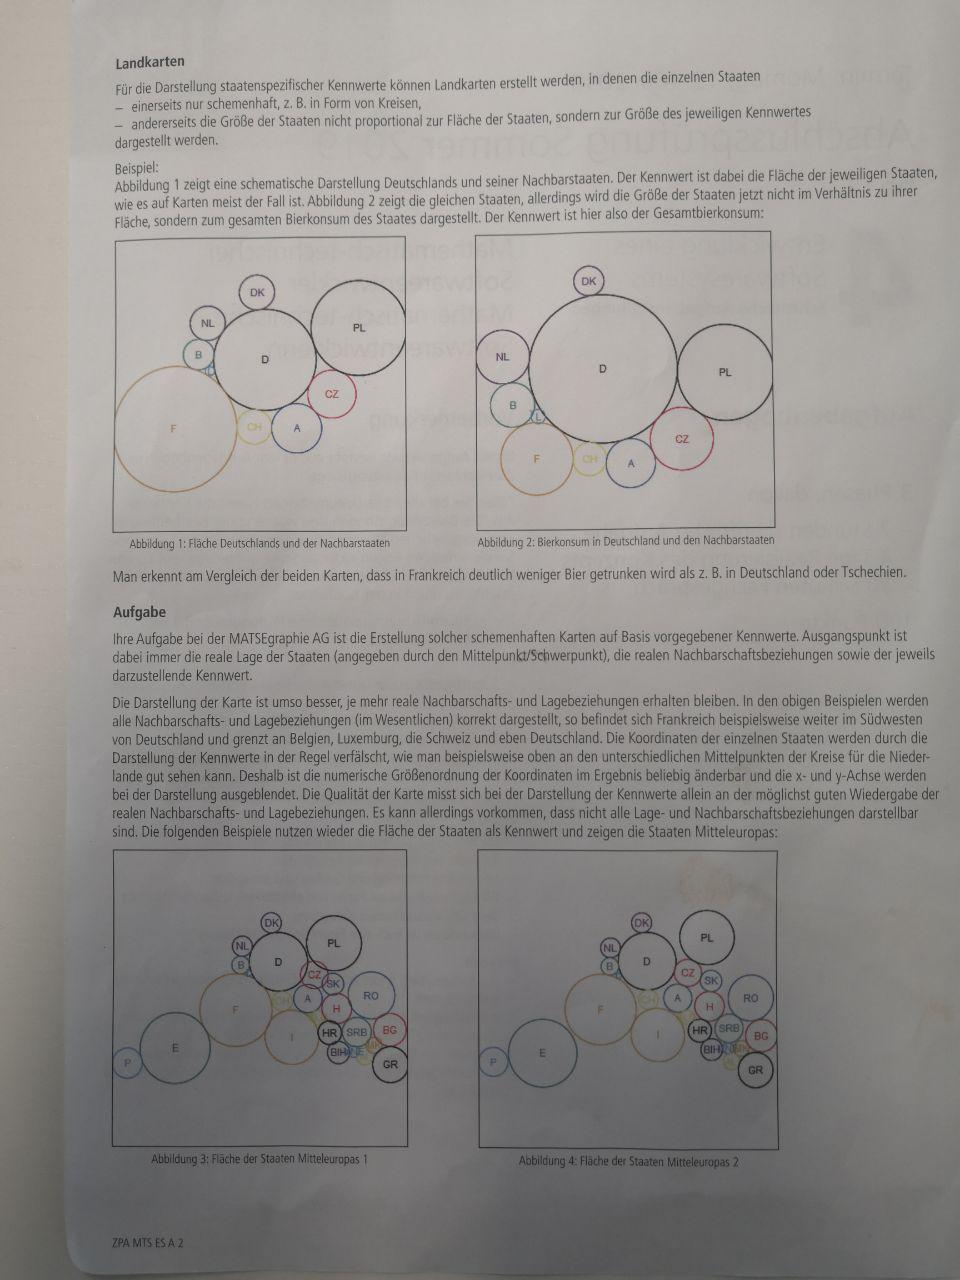
\includegraphics[width=0.8\textwidth,]{./aufgabenstellung/2.jpg}
\end{figure}

\begin{figure}[htb]
    \centering
    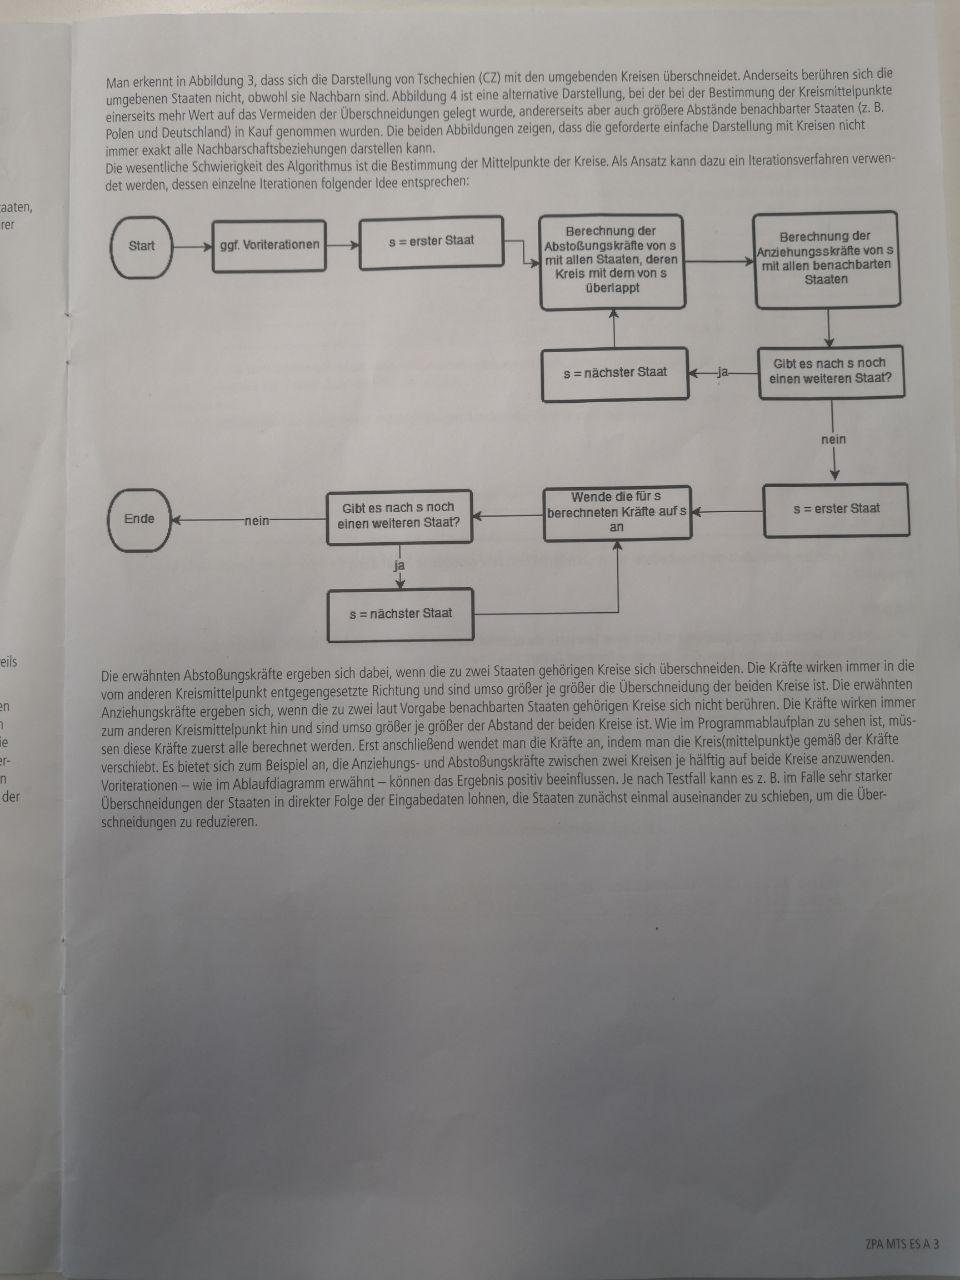
\includegraphics[width=0.8\textwidth,]{./aufgabenstellung/3.jpg}
\end{figure}

\begin{figure}[htb]
    \centering
    
\includegraphics[width=0.8\textwidth,]{./aufgabenstellung/4.jpg}
\end{figure}

\begin{figure}[htb]
    \centering
    
\includegraphics[width=0.8\textwidth,]{./aufgabenstellung/5.jpg}
\end{figure}

\begin{figure}[htb]
    \centering
    
\includegraphics[width=0.8\textwidth,]{./aufgabenstellung/6.jpg}
\end{figure}

\begin{figure}[htb]
    \centering
    
\includegraphics[width=0.8\textwidth,]{./aufgabenstellung/7.jpg}
\end{figure}

\begin{figure}[htb]
    \centering
    
\includegraphics[width=0.8\textwidth,]{./aufgabenstellung/8.jpg}
\end{figure}
